%%% Thesis Introduction --------------------------------------------------
\chapter{Introduction}
\ifpdf
    \graphicspath{{Introduction/IntroductionFigs/PNG/}{Introduction/IntroductionFigs/PDF/}{Introduction/IntroductionFigs/}}
\else
    \graphicspath{{Introduction/IntroductionFigs/EPS/}{Introduction/IntroductionFigs/}}
\fi

Internet has become the predominant mode of communication in the modern
societies of our times. Currently, 1/3 of earth population is connected to the
Internet~\cite{itufacts2011}, while Internet-related business is estimated to
account for 3.4\% of the global GDP~\cite{duRausas:2011un}. In paraller, a large
fraction of our everyday social life requires network/Internet connectivity.
Regardless the vital role of computer networking in our life, its strong
backwards compatibility ties create a gap on our ability to evolve functionality
in order to fulfil current resource short-term requirements. As a result,
although the social setting requires novel functional properties from its global
network, it is rather difficult to provide it, without disconnect a portion of
it.

My work focuses on the evolvability problem of modern networks. The key idea of
this work focuses on ways to evolve computer network functionality through
the control plane. In this dissertation we argue the thesis that: 

\begin{quotation}
  Computer network should compat the problem of network ossification through
  context-aware evolved control planes, in order to provide new properties to
  their inter-connecting fabric. Such novel control plane implentations should focus
  on the requirements of the deployment environment and customly understand and
  fit their properties and functionalities. Such approach have to be
  deployed on the edges in order to obey the end-to-end principle.  
\end{quotation}

For the remainder of this introduction we justify the importance of this thesis. In
section \ref{sec:intro:motivations} we present in details some of the limitation
that current Internet faces and the inherent limitations of current architecture
in terms of evolvability. In section \ref{sec:intro:contributions}, we
list briefly the main contributions of this thesis and in section
\ref{sec:intro:outline}, we present briefly the content of each chapter of the
thesis. Finally, in section \ref{sec:intro:pubs} we list the publications
relating to the content of this thesis. 

% Todays Internet depends to a great extend on protocols and systems designed by
% its creators from the 70's. The requirement for wide heterogeneity and backwards
% compatibility reduces our ability to innovate and evolve current network
% systems. In parrallel though, computer networks are currently a significant
% asset for the development of humanity, a state which imposes a set of
% multi-functional requirements over their deployment. The thesis of this
% dissertation is : 
% \begin{quote}
% Modern computer networks can enhance their ability to provide better user experience through
% control plane evolution. By enhancing the control plane of an SDN architecture with user
% requirement, we can enable optimal resource allocation. 
% \end{quote}
% 
% \begin{quotation}
% In the recent years, the Internet has met an incredible development in terms of
% infrastructure as well as connectivity. This development has been driven by two
% main causes: the significant reduction of the cost of network-enabled device and
% the subsequent widespread adoption from users and
% the wider utilization from companies of the Internet as a medium to interconnect and
% expand their market. Although significant, Internet development has been highly
% asymetric. The capacity of the core of the Internet has increased
% exponentially over the recent years and routing has become stable. 
% As a result, the network bottleneck has moved to the edges of the Internet, a
% point where link upgrades have a significantly higher aggregate cost and access 
% technologies have seen little innovation.
% In this work, I argue that edge networks performance is further reduce due to
% a great extend to the way many internet scale protocols are deployed.
% Further, I believe that in order to handle more efficiently
% resources in the edges, functionality of network devices should be customized to
% the needs of the specific environment and network processing should be developed
% over newer abstractions, that match the flow primitives of the specific
% environment. In this work I focus in the case of home networking and I present
% a number of novel network designs that leverage the ability to control and use
% home networks.
% \end{quotation}

% In the introduction I think it is important to mention the following points:
% % I am planning to present 2 main points:
% \begin{itemize}
% \item The core of the Internet is highly optimized and can perform really
% well the task of packet forwarding end-to-end. Although the programmability
% of the core is restricted due to the low cost principle and the high
% multiplexing of network connections. On the other hand, edge
% networks exhibit lower connection multiplexing which make programmability 
% to be handle using restricted resources. Further, in the edges we are able 
% to integrate in the
% packet processing process useful input from the users. There a number of
% measurement studies that present this differentiation both for the ADSL/cable
% (Netanalyzer, bufferbloat, ADSL measurement studies) world, as well as 3g 
% (e.g. 3gtest).
% \item The concept of network programmability is not a new concept. It has already
% been discussed in different forms (e.g. ATM controllers/switchlets, active networks) 
% which though never manage to get deployed in the real world. I need to discuss
% for the most significant cases, why these mechanisms failed to meet their
% requirements and why the SDN approach solves some of their problems. 
% \item An additional problem that I should discuss in this chapter is the
% different abstractions perceived by network applications and service
% providers. This difference in abstractions result in a significant loss of
% information that could potentially be used by both sides in order to optimize
% network utilisation.
%
% \end{itemize}
%%% ----------------------------------------------------------------------
\section{Motivation}
\label{sec:intro:motivations}

\subsubsection*{Conputer network evolution}

\begin{figure}[ht]
\centering
\subfigure[global mobile traffic trend]{
    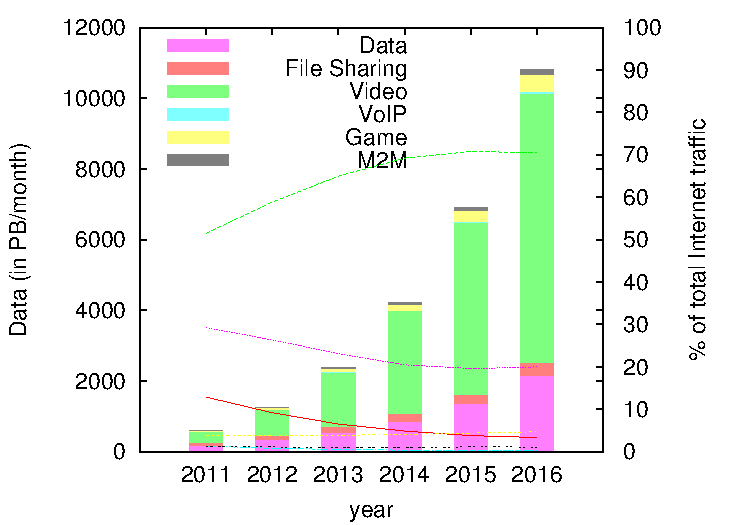
\includegraphics[width=0.45\textwidth]{mobile}
    \label{fig:internet}
}
\subfigure[global Internet traffic trend]{
    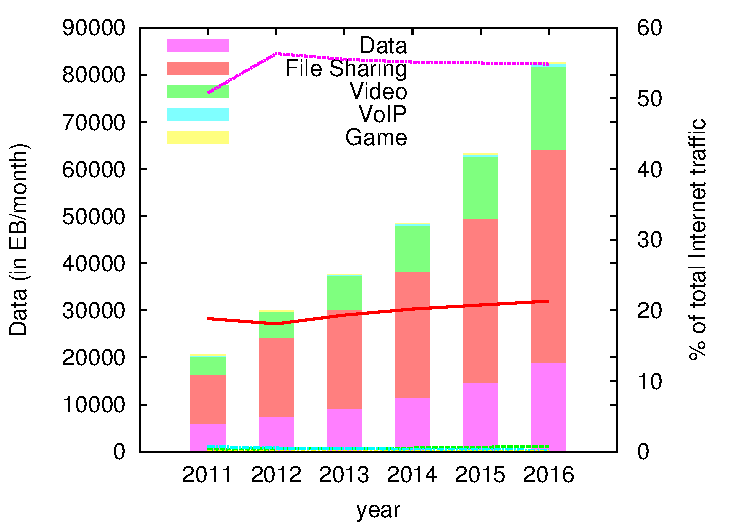
\includegraphics[width=0.45\textwidth]{internet}
    \label{fig:mobile}
}
\caption{Cisco Visual Network Index reports on global network
  traffic per application. Subfigure~\ref{fig:internet} provides details on the global Internet
  traffic trends, while Subfigure~\ref{fig:mobile} focuses on Mobile Internet
  traffic.}
\label{fig:internet_applications}
\end{figure}


\begin{table}
\begin{center}
\begin{tabular}{ | l | c c c c | }
  \hline
  Application  & rate & latency & jitter  & \# connections \\
  \hline
  web          & 0    & 0       & 0      & 0\\
  video        & 0    & 0       & 0      & 0\\
  p2p          & 0    & 0       & 0      & 0\\
  voip         & 0    & 0       & 0      & 0\\
  game         & 0    & 0       & 0      & 0\\
  \hline
\end{tabular}
\end{center}
\caption{Network performance requirement for a set of popular traffic classes.}
\label{tbl:application_requirement}
\end{table}



% a historical prespective on computer networks 
One of the ideas that formed the subjective condition of the digital revolution
of our era, was the concept of computer networking. The initial goal of this
concept was to develop a new communication architecture that would allow
continuous communication over a redundant network, even when a significant
number of vertex was destroyed.  The main building block of computer networks is
the idea of packet-switched networks~\cite{Licklider1963}.  This idea gave birth
to the pioneer of today's Internet, the {\it ARPANET}~\cite{Mills:1987tt},
allowing for the first time in computing history communication between multiple
computers over a mess network. The initial set of applications
that were standardised where : e-mail~\cite{RFC0561},
ftp~\cite{RFC0354} and voice~\cite{RFC0741}. This initial implementation was
later replaced by the NSFNET in the 80's, which finally devolved in today's
Internet. Additionally, the first transition to the NSFNET gave birth to the 
currently default protocol suite of TCP/IP~\cite{Clark:1988}, which has
seen minimum changes on its semantics and format since then.

% why computer networking is successful from the user perspective
Since the time of the ARPANET, computer networks have seen a significant
elevation on their role in the social apparatus of our world due to a number of
reasons. One of the most important trends, that boost their role, was the radical
reduction in cost, size and capabilities of network-enabled personal
computers, following Moore's Law model. In addition, the programmable nature of
the computer CPU, makes it an elegant platform to develop applications that
introduce seamlessly new functionalities. Nowadays, programmable CPUs are
integrated in a number of multipurpose devices, like mobile phones, display
devices etc, while personal computers, with their ability to transform in size,
introduce new personal computers concepts, such as laptops, tablets and other.
As a result, the paradigm of one computer per household of the 90's rapidly
shifted to the paradigm of multiple devices per user, replacing
a number of everyday single-purpose devices~\cite{Dholakia:2006vn}.  On one hand, this
augmentation in computational devices requires new modes of communication that
allow devices to share consistently state, driving a significant development in
computer network technologies. A number of network-enabled applications are
developed to address these requirements, while new network concepts are
introduced like home networks and hotspots. On the other hand, the elevated role
of computer networks and the introduction of the cloud computing paradigm,
introduce a number of internet-wide services with a global scope. These new
applications introduce a number of new assumptions on performance and connectivity
over the Internet abstraction. 

% why computer become important for the global economy too? 
In parallel with the development of the personal computer paradigm, computer
network are widely adopted as an integral asset for industry.
Currently the Internet produces 4,3\% of the global GDP. Computer Networking
and the Internet, provide the middleware to interconnect modern multinational
businesses. In the business domain computer network have become popular and
important for two main reasons: computer networks provide a cheap and fast
medium communication medium to interconnect the business logic, and the provide
a global medium to provide content to users. The adaptation of computer network
has further augmented through the utilisation of the cloud as a medium to
offload infrastructures to 3rd party cloud providers, reducing to a great extend
the cost of running services in house.\todo{add a reference to the value of the
cloud industry.} 

% How computer application mix looks in the wire? 
This wide adaptation of computer networks has introduce a number of new use cases and
applications for computer networks. Such applications introduce new assumptions over the
network abstraction. Further the popularity of network applications has a high churn over
the years, making longterm resource allocation through networking planning difficult.  In order to exhibit this trend,
we plot in Figure~\ref{fig:internet_apllications} the global prediction on traffic volumes
per applications for five years. We use data from cisco visualization index white
papers~\cite{Mobile:2012vd,Cisco:2012wu}. In histogram we can see that network traffic is
expected to increase an order of magnitude for the mobile environment, while the global
Internet traffic is expected to increase four times. In parallel, this volume increase is
uneven between traffic classes. File sharing services are expected to reduce their share
of the total volume, replaced by web and video delivery services. 

% what about the application requirements 
The problem of resource allocation is further augmented by the diverse nature of network
applications. In order to describe better the impact of these traffic changes, we list in
Table~\ref{tbl:application_requirement}, some key properties and requirements for each
traffic class. We can see in the list that applications in general have pretty diverse
properties and their requirements are difficult to fulfil during congestion. 

% How does the network look like on the edge. 
High diversity is also observed on the connection medium of the computer
networks. Currently, ethernet is currently the predominant link layer protocol
in the Internet. This dominance didn't occur since the beginning of computer
network. The main philosophy of the OSI protocol, and in respect of the TCP/IP
protocol, was the bstraction of the link layer details in order to hide the
running war between the different technologies (ATM, Token Ring). In the 80's
the low cost difference of Ethernet establish it as the leader of the market
ever since. As a result, this monoculture in the link layer, lead to the
standarization of the protocol as the de-facto link layer protocol. Since then,
although the Ethernet abstraction is global, the link layer technologies are
diverse, Introducing a number of different mediums in the Ethernet abstraction.
Currently Ethernet is exposed over coper and optical links, as well as
off-licence radio frequencies and mobile networks. Although the Ethernet
abstraction is persistent among all these mediums, the properties of the link
are diverse and difficult to keep the performance abstraction consistent.

In respect, the Internet is a highly heterogeneous 


\subsubsection{Computer network ossification}

% how does computer networks look like, How the Internet looks like?

% Introduce the reason behind protocol ossification and computer network
% evolution limitations 

% Some concrete examples of how computer networks are insufficient 

Further, the connectivity costs have reduced to a great extend, allowing
intermittent user connectivity.  Additionally, Internet since its first days,
through its simple network abstraction and it ability to self-configure and
self-heal, provides an excellent medium to interconnect heterogenious devices
and provide the connecting medium for a number of services. A connecting entity
is solely required to implement a TCP/IP stack and peer with a forwarding
entity, in order to reach any exposed Internet service.  Because of these
properties, there is a long discussion in govermental level to proclaim Internet
connectivity as a fundamental human right~\cite{klang2005human}.

% What are the communcation pattern of modern Internet?  

% How the communcation medium has changed? 

% wrap-up - Things are tricky. 

Currently, the set of Internet-wide services over the Internet in the last
decade increased exponentially. This increase in internet use cases introduced
in the network a number of new performance requirements which made traditional
network resource allocation mechanisms and network planning innefective.

In computer network literature a number of clean slate architectures has been
introduced that can address the hard problem of resource allocation, through the
design of new protocols. 
The type of the provided is diverse and thus they require
from the network diverse properties. 

\todo{Add a case for Amdahl's law.}

\section{Contributions}
\label{sec:intro:contributions}

\section{Outline}
\label{sec:intro:outline}

\section{Publications}
\label{sec:intro:pubs}

%%% Local Variables: 
%%% mode: latex
%%% TeX-master: "../thesis"
%%% End: 
